\documentclass[12pt]{beamer}
\usetheme{CambridgeUS}
\usepackage[utf8]{inputenc}
\usepackage[spanish]{babel}
\usepackage{amsmath}
\usepackage{amsfonts}
\usepackage{amssymb}
\usepackage{graphicx}

\author{Kevin Steven García \\ Cesar Andres Saavedra}
\title{TRABAJO 2 \\ TEOREMA CENTRAL DEL LIMITE \\ PRUEBAS DE NORMALIDAD}
%\setbeamercovered{transparent} 
%\setbeamertemplate{navigation symbols}{} 
%\logo{} 
\institute{Universidad del Valle \\ Estadística \\ Simulación Estadística} 
\subject{} 
\date{Mayo 2018}


\begin{document}

\begin{frame}
\titlepage
\end{frame}




\begin{frame}
\frametitle{Simulación distribución Poisson($\lambda=1$) }
\begin{figure}
\centering
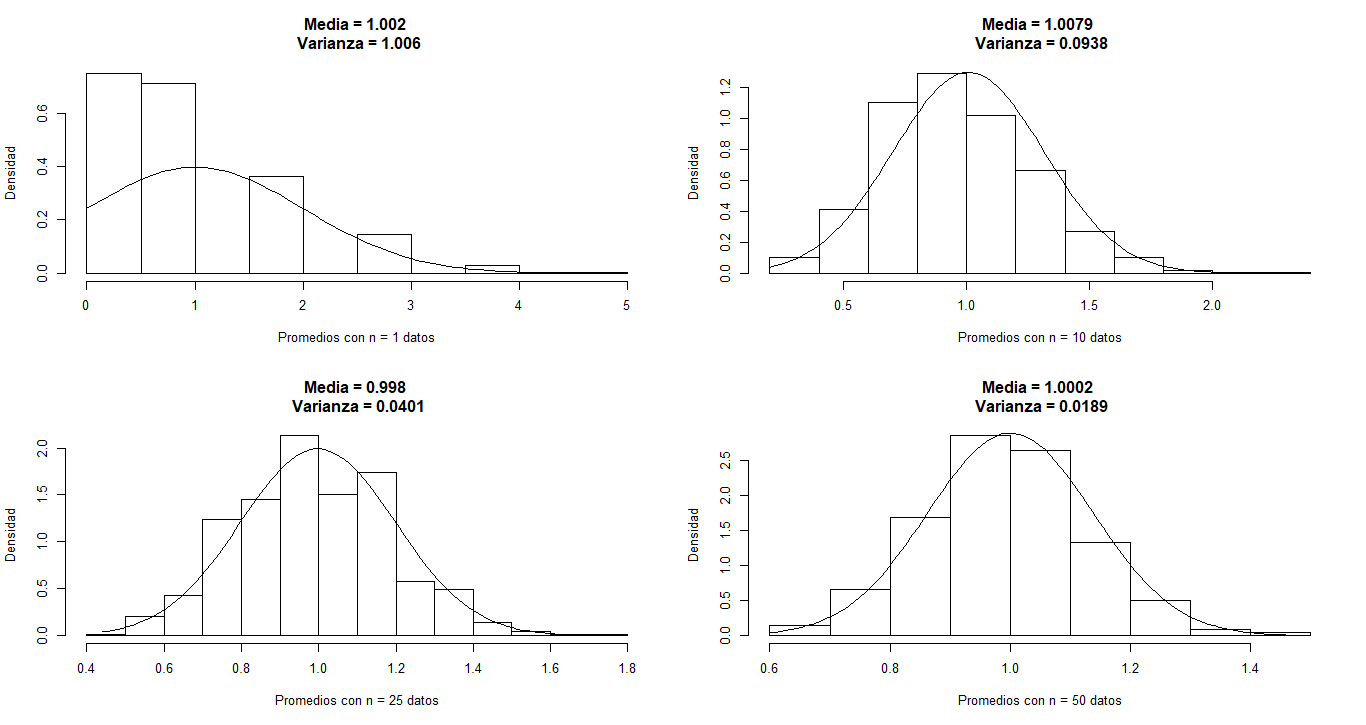
\includegraphics[scale=0.26]{imagenes/pois1.png}
\caption{Simulación y gráfica de la distribución de la media muestral para distintos valores de n}\label{figura2}
\end{figure}
\end{frame}

\begin{frame}
\frametitle{Simulación distribución Poisson($\lambda=5$) }
\begin{figure}
\centering
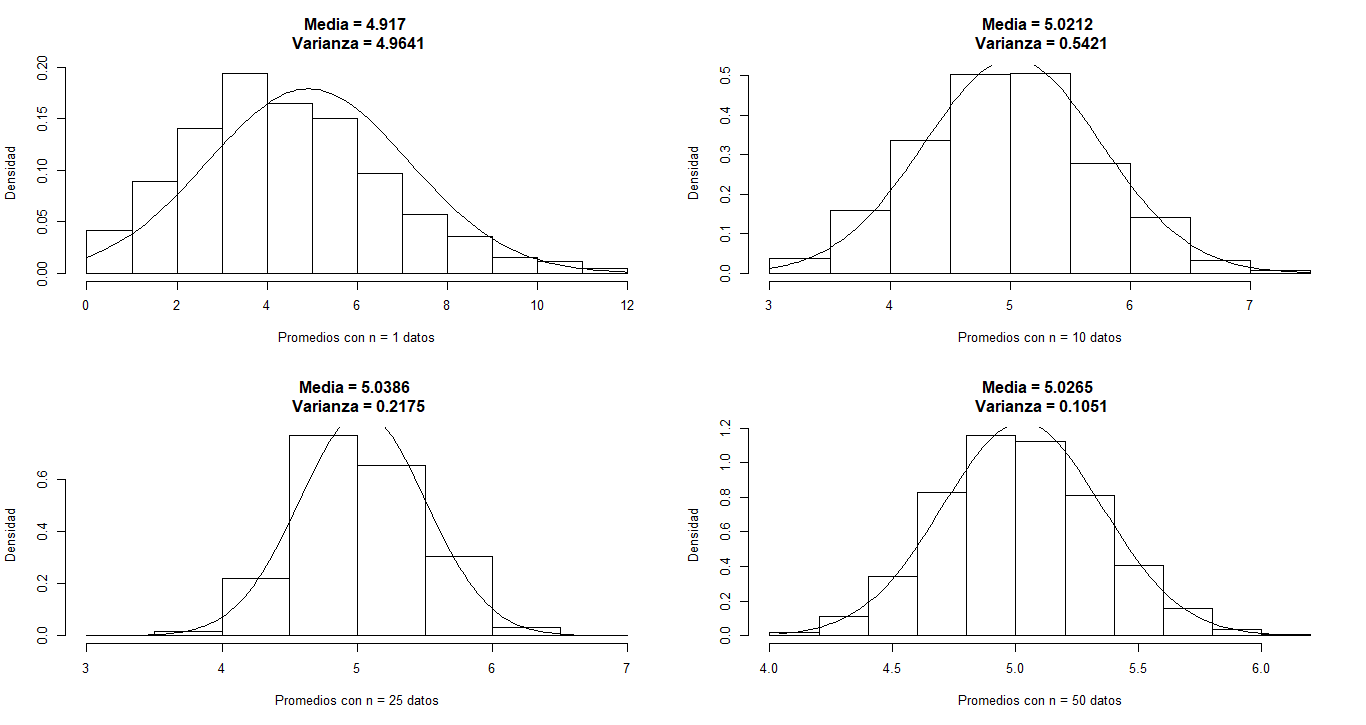
\includegraphics[scale=0.26]{imagenes/pois5.png}
\caption{Simulación y gráfica de la distribución de la media muestral para distintos valores de n}\label{figura2}
\end{figure}
\end{frame}

\begin{frame}
\frametitle{Simulación distribución Poisson($\lambda=10$) }
\begin{figure}
\centering
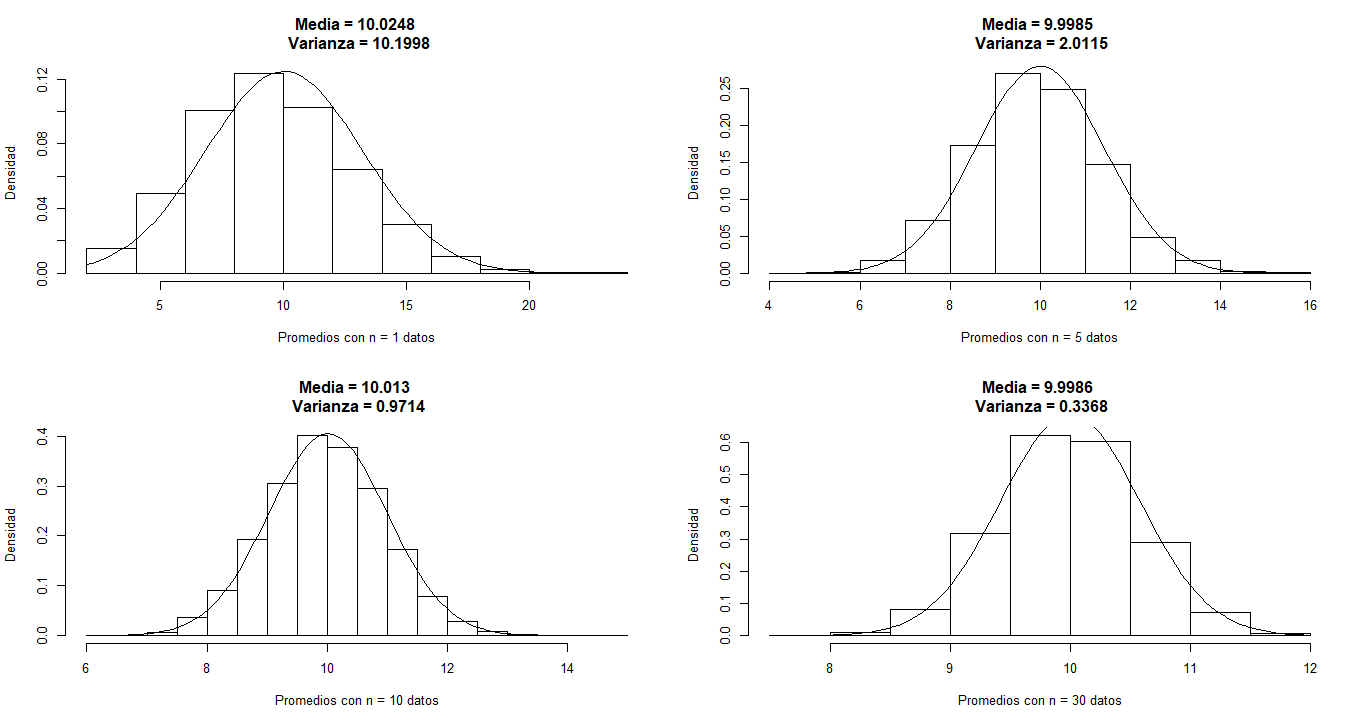
\includegraphics[scale=0.26]{imagenes/pois10.png}
\caption{Simulación y gráfica de la distribución de la media muestral para distintos valores de n}\label{figura2}
\end{figure}
\end{frame}

\begin{frame}
\frametitle{Simulación distribución Logística($\alpha=0,\beta=1$) }
\begin{figure}
\centering
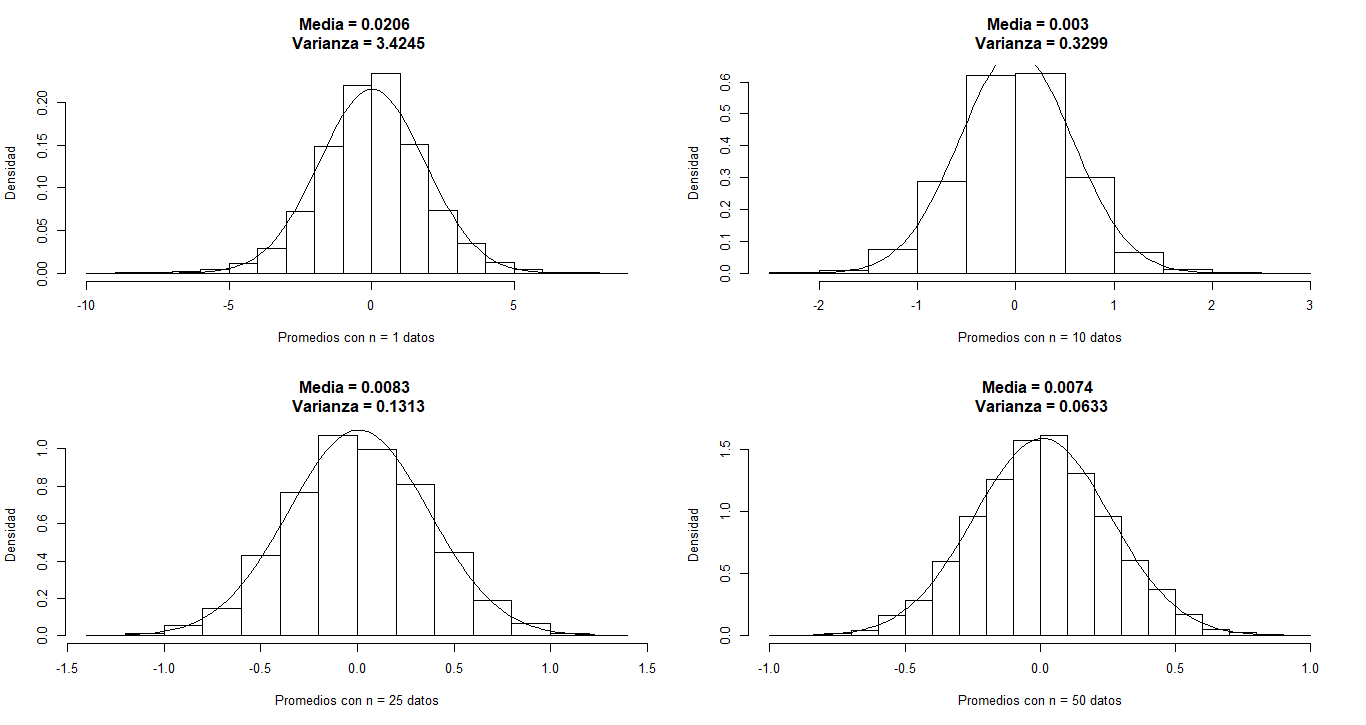
\includegraphics[scale=0.26]{imagenes/logis01.png}
\caption{Simulación y gráfica de la distribución de la media muestral para distintos valores de n}\label{figura2}
\end{figure}
\end{frame}

\begin{frame}
\frametitle{Simulación distribución Logística($\alpha=9,\beta=4$) }
\begin{figure}
\centering
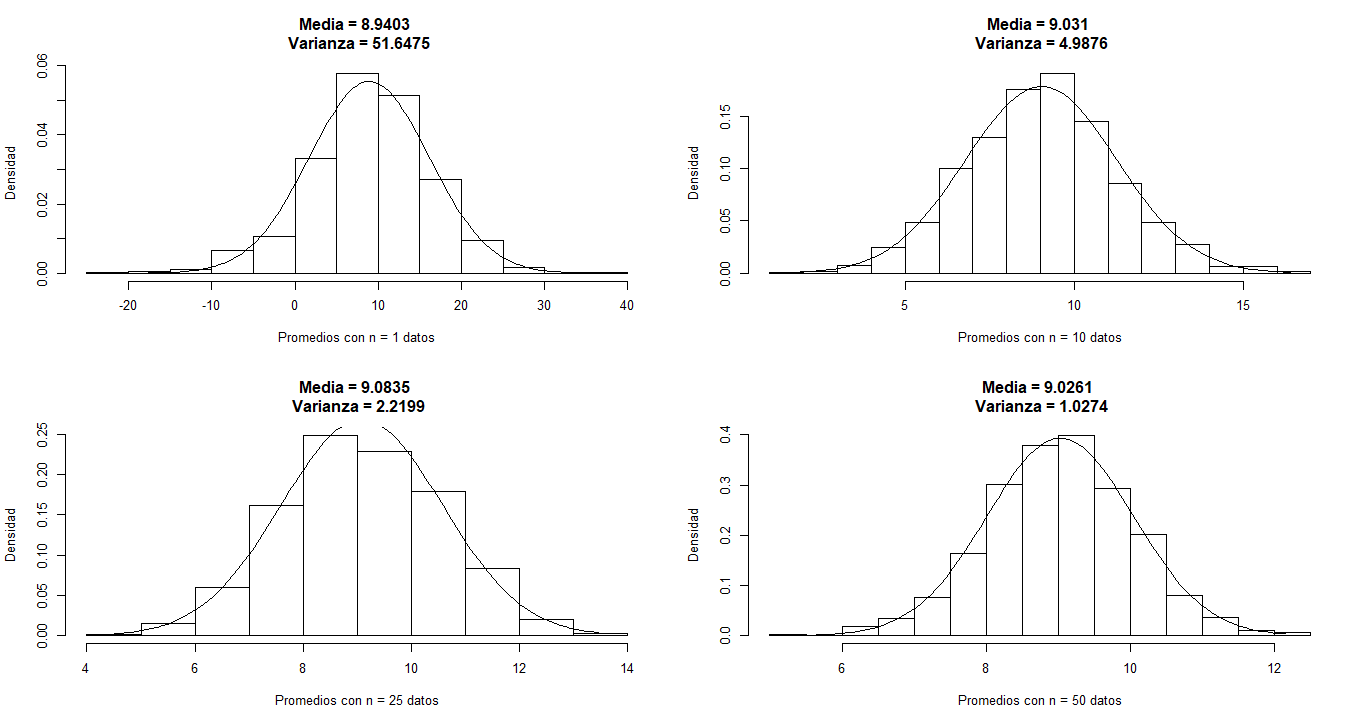
\includegraphics[scale=0.26]{imagenes/logis94.png}
\caption{Simulación y gráfica de la distribución de la media muestral para distintos valores de n}\label{figura2}
\end{figure}
\end{frame}

\begin{frame}
\frametitle{Simulación distribución Logística($\alpha=15,\beta=6$) }
\begin{figure}
\centering
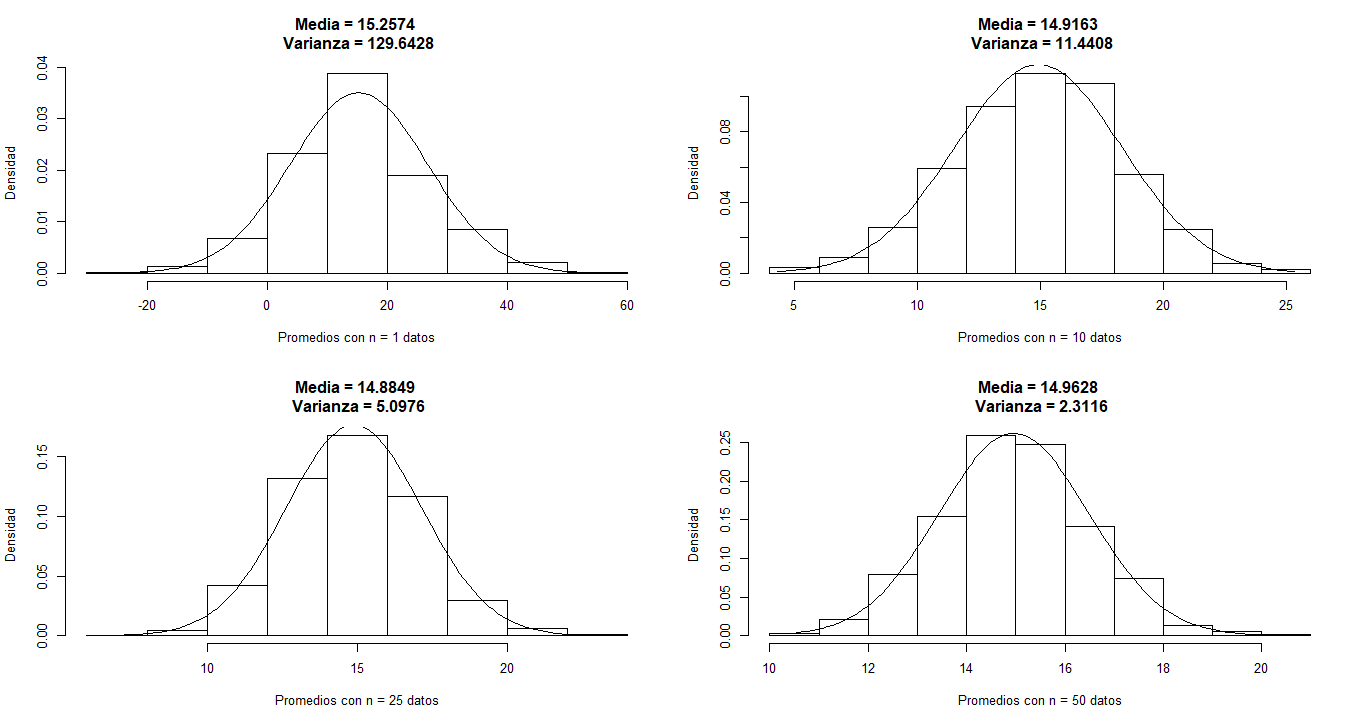
\includegraphics[scale=0.26]{imagenes/logis156.png}
\caption{Simulación y gráfica de la distribución de la media muestral para distintos valores de n}\label{figura2}
\end{figure}
\end{frame}


\begin{frame}
\frametitle{Resultados prueba de Cramér-Von Mises para la distribución Poisson}
~\\ \textbf{Para los cuales esta prueba plantea las hipotesis:}
$$H_{0}:f(x,\theta)=f_{0}(x,\theta)$$
$$H_{1}:f(x,\theta)\neq f_{0}(x,\theta) $$ 

~\\ \textbf{Para la cual se tiene como estadístico de prueba a:}
$$ W = \frac{1}{12n} + \displaystyle\sum_{i=1}^N [P_i - \frac{2_i - 1 }{2n}] $$
\end{frame}

\begin{frame}
\frametitle{Resultados prueba de Cramér-Von Mises para la distribución Poisson}
\begin{figure}
\centering
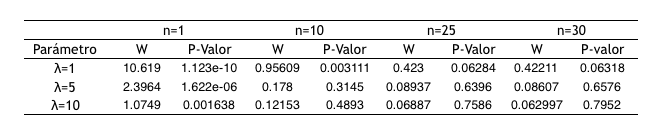
\includegraphics[scale=0.75]{imagenes/bpois.png}
\caption{Comparación resultados prueba de Cramér-Von Mises}\label{figura2}
\end{figure}
\end{frame}

\begin{frame}
\frametitle{Resultados prueba de Cramér-Von Mises para la distribución Logística}
\begin{figure}
\centering
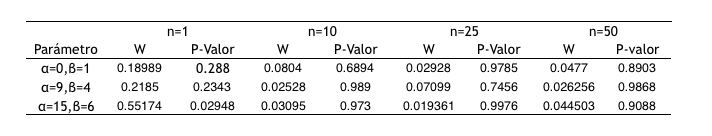
\includegraphics[scale=0.75]{imagenes/blogis.png}
\caption{Comparación resultados prueba de Cramér-Von Mises}\label{figura2}
\end{figure}
\end{frame}
\end{document}